\chapter{PSD探测单元模块大动态范围读出方案的设计与验证}
\label{ch:large_dynmaicrange}
PSD需要探测$Z=1~20$的相对论重离子,而入射重离子在PSD塑闪条中的沉积能量近似正比于$Z^2$(见\ref{sec:psd_principle})。
\begin{figure}[tb]
	\centering
	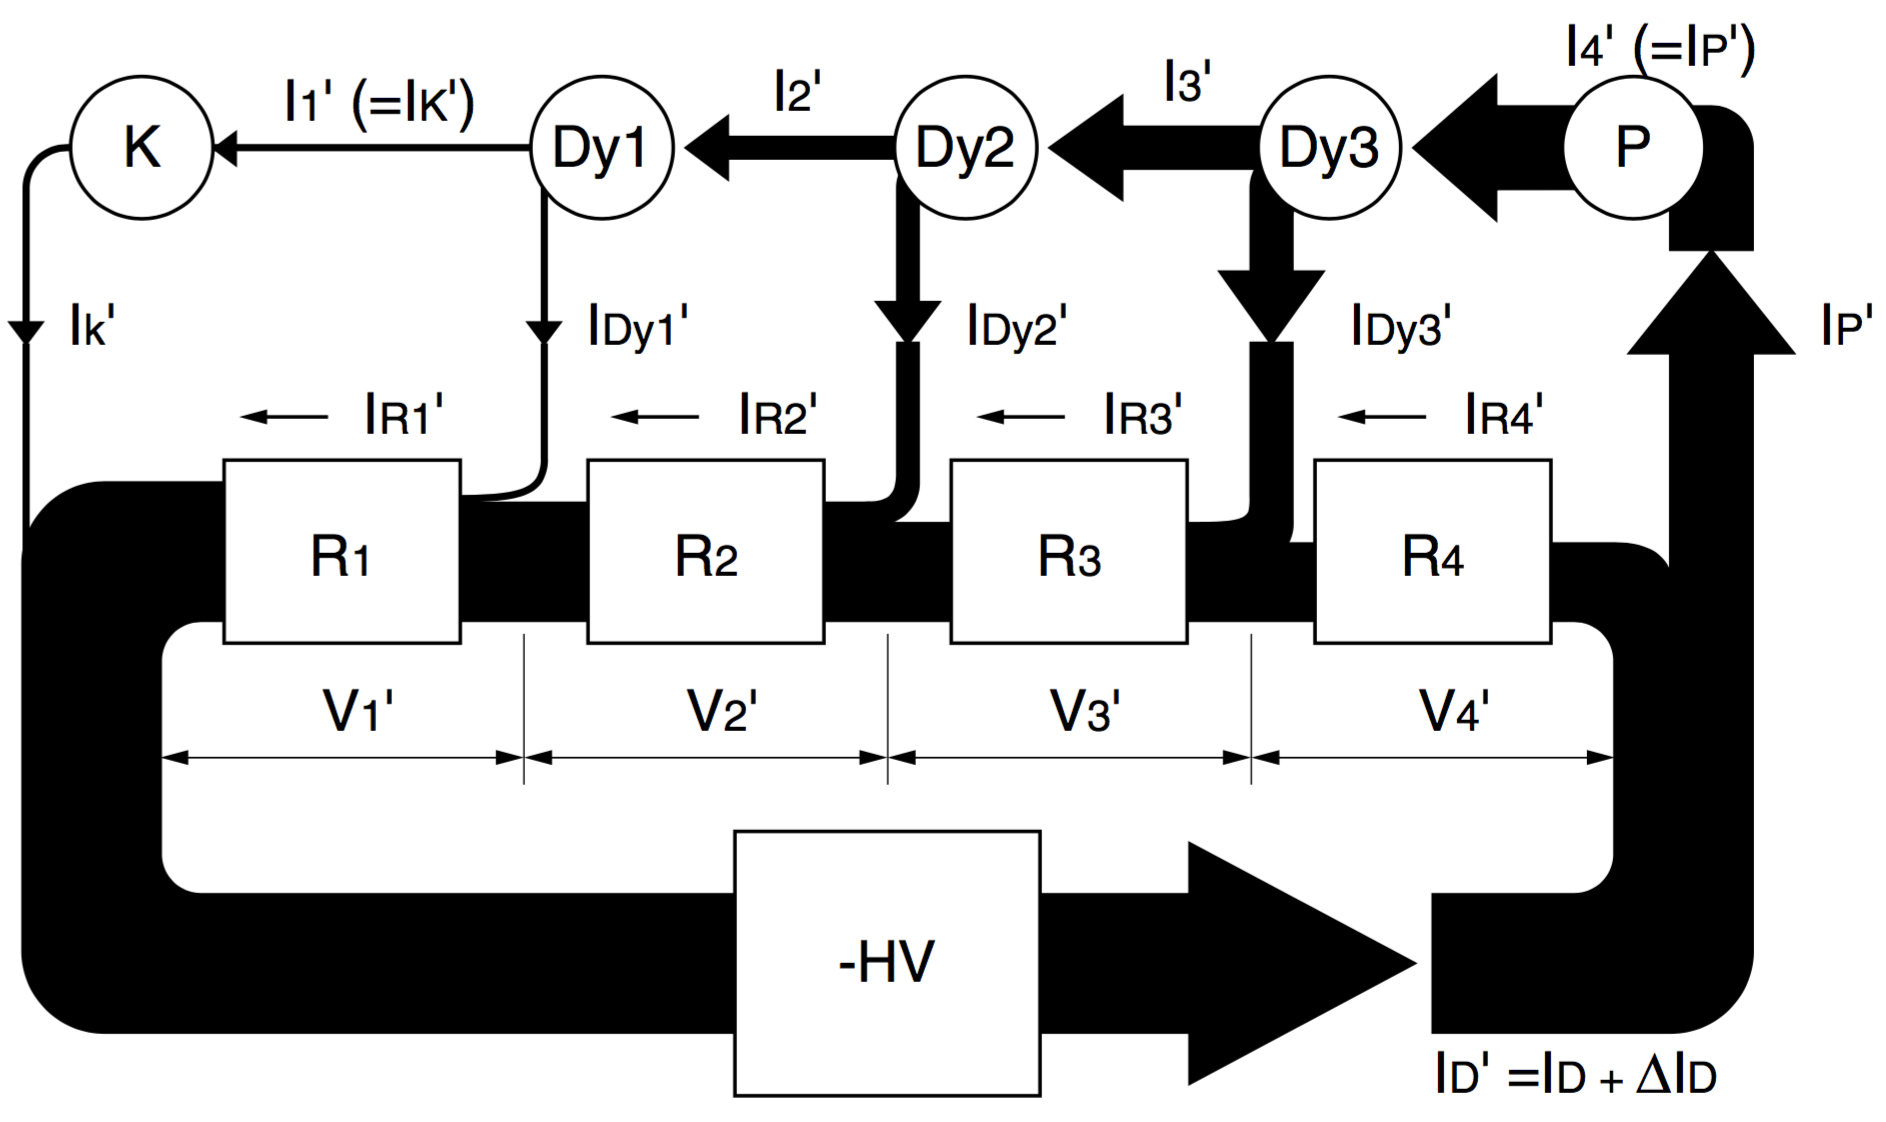
\includegraphics[width=0.9\textwidth]{chap/dynamic_range/fig/pmt_current_distribution_hamamatsu}
	\caption{Caption here}
	\label{fig:figure1}
\end{figure}
\section{重离子在塑料闪烁体中的光产额}
\label{sec:ch3:light_yield}

\section{PSD动态范围需求的估算}

\section{大动态范围读出方案的设计}
\subsection{设计思路}
\subsection{打拿极的选择}
\subsection{分压器电路的设计}

\section{大动态范围读出方案的原理验证}
\subsection{LED的测试}
\subsection{宇宙线的测试}
\subsection{中能轻核束流的测试}